\documentclass[beamer,tikz,preview]{standalone}
%\documentclass{beamer}

\setbeamertemplate{navigation symbols}{}
\usepackage{tikz}
\usepackage{tikz-cd}
\usepackage{color}

\definecolor{MyColor}{HTML}{1565C0}


\begin{document}

\begin{frame}
    \begin{center}
    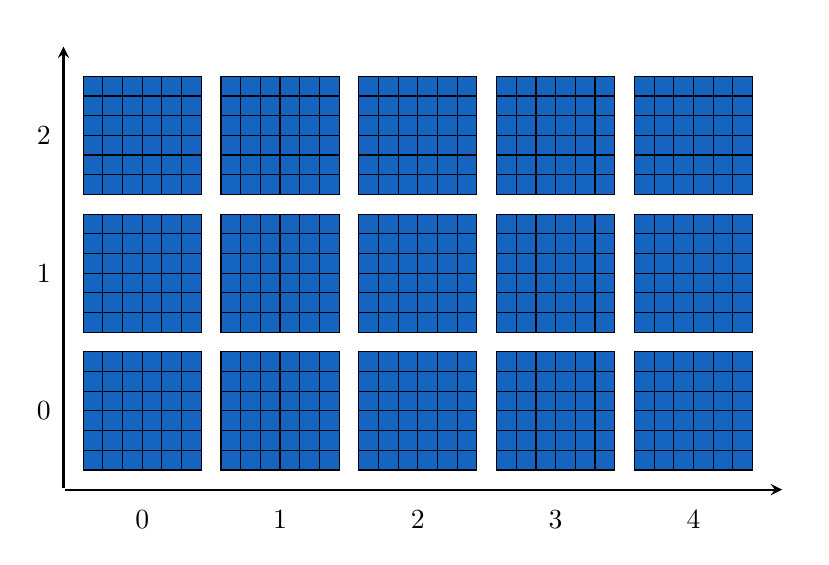
\begin{tikzpicture}
      % Parameters
      \pgfmathsetmacro{\length}{1.5}
      \pgfmathsetmacro{\rows}{6}
      \pgfmathsetmacro{\spacing}{0.25}
      \pgfmathsetmacro{\w}{\length/\rows}
  
      % Axes 
      \node(origin) at (-2*\length/\rows,-\length) [inner sep=0pt] {};
      \node(xaxis) at (5*\length+5*\spacing,-\length) {};
      \node(yaxis) at (-2*\length/\rows,2*\length+5*\spacing) {};
      \draw[-stealth,thick] (origin) -- (xaxis);
      \draw[-stealth,thick] (origin) -- (yaxis);
  
      % x-axis labels
      \foreach \k in {0,...,4}{
        \node at (\k*\length+\k*\spacing+2*\length/\rows, -\length-1.5*\length/\rows) {\k};
      }
      
      % y-axis labels
      \foreach \k in {0,...,2}{
        \node at (-3*\length/\rows,-2*\length/\rows + \k*\length + \k*\spacing) {\k};
      }
  
    

    % Bottom row (LCS)
    \foreach \k in {0,...,4}{
      \pgfmathsetmacro{\xbase}{(\length+\spacing)*\k}
      \pgfmathsetmacro{\ybase}{0}
      \foreach \i in {1,...,\rows}{
        \foreach \j in {1,...,\rows}{
          \pgfmathsetmacro{\x}{\xbase+(\j-1)*\length/\rows}
          \pgfmathsetmacro{\y}{\ybase-(\i-1)*\length/\rows}
          \pgfmathsetmacro{\ik}{\i+\k}
          \pgfmathsetmacro{\compj}{\j+0}
          \ifboolexpr{ test {\ifnumequal{\i}{\j}} }
            {\draw[fill=black] (\x,\y) -- ++(-\w,0) -- ++(0,\w) -- ++(\w,0) -- cycle;}
            {\ifboolexpr{ test {\ifdimless{\compj pt}{\ik pt}}}
              {\draw[fill=white] (\x,\y) -- ++(-\w,0) -- ++(0,\w) -- ++(\w,0) -- cycle;}
              {\ifboolexpr{ test {\ifnumequal{\j}{\i+\k}}}
                {\draw[fill=MyColor] (\x,\y) -- ++(-\w,0) -- ++(0,\w) -- ++(\w,0) -- cycle;}
                {\draw[fill=MyColor] (\x,\y) -- ++(-\w,0) -- ++(0,\w) -- ++(\w,0) -- cycle;}
              }
            }
        }
      }
    }

    \pgfmathsetmacro{\xbase}{\length+\spacing}
    \pgfmathsetmacro{\ybase}{\length+\spacing}
    \foreach \i in {1,...,\rows} {
      \foreach \j in {1,...,\rows} {
        \pgfmathsetmacro{\x}{\xbase+(\j-1)*\length/\rows}
        \pgfmathsetmacro{\y}{\ybase-(\i-1)*\length/\rows}
        \ifboolexpr{ test {\ifnumequal{\i}{\j}}}
          {\draw[fill=black] (\x,\y) -- ++(-\w,0) -- ++(0,\w) -- ++(\w,0) -- cycle;}
          {\ifboolexpr{ test {\ifnumless{\j}{\i+2}}}
            {\ifboolexpr{ test {\ifnumequal{\i}{1}} or test{\ifnumequal{\j}{6}} }
              {\draw[fill=MyColor] (\x,\y) -- ++(-\w,0) -- ++(0,\w) -- ++(\w,0) -- cycle;}
              {\draw[fill=white] (\x,\y) -- ++(-\w,0) -- ++(0,\w) -- ++(\w,0) -- cycle;}
            }
            {\draw[fill=MyColor] (\x,\y) -- ++(-\w,0) -- ++(0,\w) -- ++(\w,0) -- cycle;}
          }
      }
    }

      % First column
      \foreach \k in {1,...,2}{
        \pgfmathsetmacro{\xbase}{0}
        \pgfmathsetmacro{\ybase}{(\length+\spacing)*\k}
        \foreach \i in {1,...,\rows}{
          \foreach \j in {1,...,\rows}{
            \pgfmathsetmacro{\x}{\xbase+(\j-1)*\length/\rows}
            \pgfmathsetmacro{\y}{\ybase-(\i-1)*\length/\rows}
            \pgfmathsetmacro{\ik}{\i+\k}
            \pgfmathsetmacro{\compj}{\j+0}
            \ifboolexpr{ test {\ifnumequal{\i}{\j}} }
              {\draw[fill=black] (\x,\y) -- ++(-\w,0) -- ++(0,\w) -- ++(\w,0) -- cycle;}
              {\ifboolexpr{ test {\ifnumless{\j}{\i}}}
                {\draw[fill=white] (\x,\y) -- ++(-\w,0) -- ++(0,\w) -- ++(\w,0) -- cycle;}
                {\draw[fill=MyColor] (\x,\y) -- ++(-\w,0) -- ++(0,\w) -- ++(\w,0) -- cycle;}
              }
          }
        }
      }
  
      % First row
      \foreach \k in {1,...,4}{
        \pgfmathsetmacro{\xbase}{(\length+\spacing)*\k}
        \pgfmathsetmacro{\ybase}{2*(\length+\spacing)}
        \foreach \i in {1,...,\rows}{
          \foreach \j in {1,...,\rows}{
            \pgfmathsetmacro{\x}{\xbase+(\j-1)*\length/\rows}
            \pgfmathsetmacro{\y}{\ybase-(\i-1)*\length/\rows}
            \pgfmathsetmacro{\ik}{\i+\k+1}
            \pgfmathsetmacro{\compj}{\j+0}
            \ifboolexpr{ test {\ifnumequal{\i}{\j}} }
              {\draw[fill=black] (\x,\y) -- ++(-\w,0) -- ++(0,\w) -- ++(\w,0) -- cycle;}
              {\ifboolexpr{ test {\ifdimless{\compj pt}{\ik pt}}}
                {\draw[fill=white] (\x,\y) -- ++(-\w,0) -- ++(0,\w) -- ++(\w,0) -- cycle;}
                {\draw[fill=MyColor] (\x,\y) -- ++(-\w,0) -- ++(0,\w) -- ++(\w,0) -- cycle;}
              }
          }
        }
      }
  
      % Generated subgroups 
      \foreach \k in {2,...,4}{
        \pgfmathsetmacro{\xbase}{\k*\length+\k*\spacing}
        \pgfmathsetmacro{\ybase}{\length+\spacing}
        \foreach \i in {1,...,\rows} {
          \foreach \j in {1,...,\rows} {
            \pgfmathsetmacro{\x}{\xbase+(\j-1)*\length/\rows}
            \pgfmathsetmacro{\y}{\ybase-(\i-1)*\length/\rows}
            \ifboolexpr{ test {\ifnumequal{\i}{\j}}}
              {\draw[fill=black] (\x,\y) -- ++(-\w,0) -- ++(0,\w) -- ++(\w,0) -- cycle;}
              {\ifboolexpr{ test {\ifnumless{\j}{\i+\k+1}}}
                {\ifboolexpr{ test {\ifnumequal{\i}{1}} or test{\ifnumequal{\j}{6}} and test {\ifnumequal{\j}{\i+\k}} }
                  {\draw[fill=MyColor] (\x,\y) -- ++(-\w,0) -- ++(0,\w) -- ++(\w,0) -- cycle;}
                  {\draw[fill=white] (\x,\y) -- ++(-\w,0) -- ++(0,\w) -- ++(\w,0) -- cycle;}
                }
                {\draw[fill=MyColor] (\x,\y) -- ++(-\w,0) -- ++(0,\w) -- ++(\w,0) -- cycle;}
              }
          }
        }
      }
  
      % Credit
      %\node at (7.5,-2.25) {{\tiny J.\ Maglione (2017)}};
      % Full citation: 
      % Joshua Maglione, Efficient characteristic refinements for finite groups, J. Symbolic Comput. 80 (2017), part 2, 511--520.
    \end{tikzpicture}
    \end{center}
  \end{frame}
  
\end{document}